\section{Ôn tập học kỳ 1}
\subsection{Đề 1}
\Opensolutionfile{ans}[ans/ans-2-HK1-DE1]
\caulc
%%==========Câu 1
\begin{ex}%[2D1N5-1] 
\immini[thm]{
	Đồ thị của hàm số nào dưới đây có dạng như đường cong hình bên?
	\choice
	{$y=-x^3+3x-1$}
	{$y=x^4-2x^2-2$}
	{$y=x^3-x+2$}
	{\True $y=x^3-x-2$}
}
{
	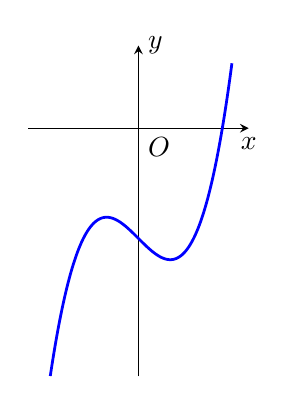
\begin{tikzpicture}[>=stealth,scale=0.7]
	\draw[->] (-2,0) --(0,0) node[below	right]{$O$} -- (2,0) node[below]{$x$};
	\draw[->](0,-4.5)--(0,1.5) node[right]{$y$};
	\draw[smooth,blue,line width=1] plot[domain=-1.6:1.7] (\x,{(\x)^3-(\x)-2});
	\end{tikzpicture}
}
\loigiai{
	Dễ thấy đồ thị hàm số đã cho là đồ thị hàm số bậc ba có hệ số $a>0$.\\
	Mặt khác đồ thị hàm số cắt trục tung tại điểm có tung độ âm nên $d<0$.\\
	Suy ra hàm số cần tìm là $y=x^3-x-2$.}
\end{ex}

%%==========Câu 2
\begin{ex}%[2H2H2-4]
Trong không gian $Oxyz$, cho các điểm $A(3;0;1),B(2;3;0),C(1;1;1)$. Sin của $\widehat{ABC}$ bằng
\choice
{$ \sqrt{\dfrac{6}{11}} $}
{$ \sqrt{\dfrac{2}{3}} $}
{$ \sqrt{\dfrac{1}{3}} $}
{\True$ \sqrt{\dfrac{5}{11}} $}
\loigiai{Ta có $\overrightarrow{BA}=(1;-3;1)$ và $\overrightarrow{BC}=(-1;-2;1)$. Do đó 
	$$\cos(\widehat{ABC})=\cos(\overrightarrow {BA},\overrightarrow {BC})=\dfrac{-1+6+1}{\sqrt{1+9+1}\cdot\sqrt{1+4+1}}=\sqrt{\dfrac{6}{11}}\Rightarrow \sin(\widehat{ABC})=\sqrt{\dfrac{5}{11}}.$$
}
\end{ex}

%%==========Câu 3
\begin{ex}%[2D3H1-4] 
Cho bảng phân bố tần số sau
\begin{center}
	\newcolumntype{P}[1]{>{\centering\arraybackslash}p{#1}}
	\begin{tabular}{|c|P{0.6in}|P{0.6in}|P{0.6in}|P{0.6in}|P{0.6in}|}
		\hline
		Giá trị & $x_1$    & $x_2$    & $x_3$    & $x_4$    & $x_5$ \\
		\hline
		Tần số &   3    &      5     &  $n+6$    & $20-n$    & 9 \\
		\hline
	\end{tabular}
\end{center}
Trong đó $ n $ là số tự nhiên và giá trị $x_4 $ là mốt duy nhất của bảng số liệu thống kê đã cho. Có bao nhiêu giá trị $n$ thỏa mãn yêu cầu?
\choice
{\True$7$}
{$6$}
{$5$}
{$4$}
\loigiai{
	Từ giả thiết $x_4$ là mốt duy nhất của bảng số liệu thống kê đã cho nên ta có
	$$\heva{& 20-n>9 \\   & 20-n>n+6}\Leftrightarrow \heva{ & n<11 \\   & n<7}\Leftrightarrow n<7.$$
	Vì $n$ là số tự nhiên nên các giá trị $n$ thỏa mãn là $0\le n<7$.
}
\end{ex}

%%==========Câu 4
\begin{ex}%[2D1H1-2]
\immini[thm]{Cho hàm số $f(x)$ có đạo hàm $f’(x)$ xác định, liên tục trên $\mathbb{R}$ và $f’(x)$ có đồ thị như hình vẽ bên. Khẳng định nào sau đây là đúng?
	\choice
	{Hàm số $f(x)$ đồng biến trên $(-\infty;1)$}
	{Hàm số $f(x)$ đồng biến trên $(-\infty;1)$ và $(1;+\infty)$}
	{\True Hàm số $f(x)$ đồng biến trên $(1;+\infty)$}
	{Hàm số $f(x)$ đồng biến trên $\mathbb{R}$}}
{\begin{tikzpicture}[>=stealth,line join=round,line cap=round,font=\normalsize,scale=0.6]
	\draw[-stealth] (-1,0)--(0,0)node[above left]{\scriptsize $O$}--(3,0)node[below]{\scriptsize $x$};
	\draw[-stealth] (0,-3)--(0,3)node[left]{\scriptsize $y$};
	\draw (-1,-2.5)--(1,0)--(2.5,2.5);
	\draw 
	(1,0) node[below]{\scriptsize $1$}
	;
	\end{tikzpicture}}

\loigiai{
	Dựa vào đồ thị hàm số $f’(x)$, ta thấy $f’(x)>0,\forall x\in(1;+\infty)$ suy ra hàm số $f(x)$ đồng biến trên $(1;+\infty)$.}
\end{ex}

%%==========Câu 5
\begin{ex}%[2D3H2-2] 
Tiền thưởng của $35$ nhân viên trong một công ty được thống kê trong bảng tần số ghép lớp sau đây (đơn vị: triệu đồng)
\begin{center}
	\begin{tabular}{|c|c|c|c|c|c|c|}
		\hline 
		\bf Lớp &$[20;24]$ &$[25;29]$&$[30;34]$&$[35;39]$&$[40;44]$& Cộng\\ 
		\hline
		\bf Tần số &$2$&$7$&$15$&$8$&$3$&$n=35$\\
		\hline
	\end{tabular}
\end{center}
Độ lệch chuẩn (kết quả làm tròn đến hàng phần trăm) bằng
\choice
{$5{,}28$}
{$6{,}43$}
{$3{,}52$}
{\True$4{,}98$}
\loigiai{
	\begin{center}
		\begin{tabular}{|c|c|c|c|c|c|c|}
			\hline 
			\bf Lớp &$[20;24]$ &$[25;29]$&$[30;34]$&$[35;39]$&$[40;44]$& Cộng\\ 
			\hline
			\bf Giá trị đại diện &$22$ &$27$&$32$&$37$&$42$& Cộng\\ 
			\hline
			\bf Tần số &$2$&$7$&$15$&$8$&$3$&$n=35$\\
			\hline
		\end{tabular}
	\end{center}
	Phương sai $$s_x^2=\dfrac{2\cdot 22^2+7\cdot 27^2+15\cdot 32^2+8\cdot 37^2+3\cdot 42^2}{35}-\left(\dfrac{2\cdot 22+7\cdot 27+15\cdot 32+8\cdot 37+3\cdot 42}{35}\right)^2.$$
	Do vậy độ lệch chuẩn $s_x=\sqrt{s^2}=4{,}98$.
}
\end{ex}

%%==========Câu 6
\begin{ex}%[2D3H2-2] 
	Cho bảng phân bố tần số ghép lớp: 
\begin{center}
	\begin{tabular}{|l|c|c|c|c|}
		\hline
		{Lớp các giá trị $x$}&{[8; 10)}&{[10; 12)}&{[12; 14]}&{Cộng}\\
		\hline
		{Tần số $n_i$}&{15}&{30}&{55}&{100}\\
		\hline
	\end{tabular}	
\end{center}
Hãy tìm số trung bình của các giá trị trong bảng trên.
\choice
{$\dfrac{69}{5}$}
{\True$\dfrac{59}{5}$}
{$50$}
{$11$}
\loigiai
{Giá trị đại diện của lớp $\left[8; 10\right)$: $c_1=\dfrac{8 + 10}{2}=9$.\\ 
	Giá trị đại diện của lớp $\left[10; 12\right)$: $c_2=\dfrac{10 + 12}{2}=11$.\\ 
	Giá trị đại diện của lớp $\left[12; 14\right)$: $c_3=\dfrac{12 + 14}{2}=13$.\\ 
	Số trung bình cộng: $\overline{x}=\dfrac{9\cdot15 + 11\cdot30 + 13\cdot55}{15 + 30 + 55}=\dfrac{59}{5}$.
}
\end{ex}

%%==========Câu 7
\begin{ex}%[2H2H2-2]
Trong không gian với hệ trục tọa độ $Oxyz$, cho ba điểm $A(1; 2;-1)$, $B(2;-1; 3)$, $C(-3; 5; 1)$. Tìm tọa độ điểm $D$ sao cho tứ giác $ABCD$ là hình bình hành. 
\choice
{$D(-2; 8;-3)$}
{$D(-2; 2; 5)$}
{$D(-4; 8;-5)$}
{\True $D(-4; 8;-3)$}
\loigiai{
	Ta có $\vec{AD}=\vec{BC}\Leftrightarrow\left(x_D-1;y_D-2;z_D+1\right)=(-5;6;-2)\Leftrightarrow\heva{&x_D-1=-5\\&y_D-2=6\\&z_D+1=-2}\\\Rightarrow D(-4;8;-3)$.}
\end{ex}

%%==========Câu 8
\begin{ex}%[2D3H1-4]
Điểm kiểm tra môn Toán của $40$ học sinh lớp 10B được thống kê trong bảng phân bố tần số sau đây (thang điểm $10$):
\begin{center}
	\begin{tabular}{|c|c|c|c|c|c|c|c|c|c|c|c|c|}
		\hline 
		\bf Điểm &$0$ &$1$&$2$&$3$&$4$&$5$&$6$&$7$&$8$&$9$&$10$& Cộng\\ 
		\hline
		\bf Tần số &$2$ &$1$&$2$&$1$&$2$&$x$&$5$&$7$&$y$&$5$&$4$& $n=40$\\
		\hline
	\end{tabular}
\end{center}
Biết rằng mẫu số liệu trên có $2$ mốt. Hãy tìm $x$ và $y$.
\choice
{$x=8$; $y=7$}
{\True$x=8$; $y=8$}
{$x=7$; $y=9$}
{$x=7$; $y=8$}
\loigiai{Tổng số học sinh là $45$ nên $x+y=16$, suy ra có ít nhất một trong hai số $x$ hoặc $y$ không nhỏ hơn $8$. Vì mẫu số liệu có 2 mốt nên $x=y=8$ thỏa mãn.
	}
\end{ex}

%%==========Câu 9
\begin{ex}%[2D1K1-3] 
Số giá trị nguyên của tham số $m$ trên sao cho hàm số $y=\dfrac{m\ln x-2m}{\ln x-m}$ đồng biến trên khoảng $(\mathrm{e};+\infty)$. 
\choice
{$2$}
{\True $1$}
{$3$}
{$4$}
\loigiai{
	Điều kiện $\ln x\neq m$.\\
	Ta có $y'=\dfrac{1}{x}\cdot\dfrac{-m^2+2m}{(\ln x-m)^2}$. Vì $\dfrac{1}{x}>0$,  $\forall x\in(\mathrm{e};+\infty)$ và $\ln x\in(1;+\infty)$,  $\forall x\in(\mathrm{e};+\infty)$.\\
	Suy ra hàm số đã cho đồng biến trên khoảng $(0;+\infty)$ khi và chỉ khi
	$$\heva{&-m^2+2m>0\\&m\notin(1;+\infty)}\Leftrightarrow\heva{&0<m<2\\&m\leq 1}\Leftrightarrow 0<m\leq 1.$$
	Vì $m$ nguyên nên $m=1$.}
\end{ex}

%%==========Câu 10
\begin{ex}%[2H2K2-2]
Tìm tọa độ điểm $M$ trên trục $Ox$ cách đều hai điểm $A(1;2;-1)$ và điểm $B(2;1;2)$. 
\choice
{$M\left(\dfrac{1}{2};0;0\right)$}
{\True $M\left(\dfrac{3}{2};0;0\right)$}
{$M\left(\dfrac{2}{3};0;0\right)$}
{$M\left(\dfrac{1}{3};0;0\right)$}
\loigiai{
	Gọi $M(x;0;0)\in Ox$.\\
	Ta có $MA=MB\Leftrightarrow MA^2=MB^2\Leftrightarrow(1-x)^2+4+1=(2-x)^2+1+4\Leftrightarrow x=\dfrac{3}{2}$.\\
	Vậy $ M\left(\dfrac{3}{2};0;0\right)$.}
\end{ex}

%%==========Câu 11
\begin{ex}%[2H2G1-3]
Cho hình chóp $S.A B C D$ có đáy $A B C D$ là hình bình hành, có độ dài các cạnh $A B=8 $; $ A C=6 $; $ S C=10 $; $ \widehat{S A D}=90^{\circ}$. Tính độ dài cạnh $S B$.
\choice
{\True$8\sqrt{2}$}
{$12$}
{$6$}
{$6\sqrt{6}$}
\loigiai{
	\immini
	{
		Ta có 
		\allowdisplaybreaks
		\begin{eqnarray*}
			&&\overrightarrow{SA}\cdot \overrightarrow{BC} = \left(\overrightarrow{SB}+\overrightarrow{BA}\right)\cdot \overrightarrow{BC}\\
			&=& \overrightarrow{SB}\cdot\overrightarrow{BC}+\overrightarrow{BA}\cdot \overrightarrow{BC}\\
			&=&  -\overrightarrow{BS}\cdot\overrightarrow{BC}+\overrightarrow{BA}\cdot \overrightarrow{BC}\\
			&=& - BS \cdot BC \cdot \cos \widehat{SBC} + BA \cdot BC\cdot \cos \widehat{ABC}\\
			%		&=&- BA \cdot BD \cdot \dfrac{CA^2+CD^2-AD^2}{2CA\cdot CD} + CB \cdot CD \cdot \dfrac{CB^2+CD^2-BD^2}{2CB\cdot CD}\\
			&=&\dfrac{-BS^2-BC^2+SC^2+BA^2+BC^2-AC^2}{2}\\
			&=&\dfrac{SC^2+BA^2-BS^2-AC^2}{2}.
		\end{eqnarray*}
	}
	{
		\begin{tikzpicture}[scale=1, font=\footnotesize, line join=round, line cap=round, >=stealth]
		\def\bc{4} % cạnh BC
		\def\ba{2} % cạnh BA
		\def\h{4} % đường cao
		\def\gocB{45} % góc B của đáy
		\coordinate[label=below left:$B$] (B) at (0,0);
		\coordinate[label=above right:$A$] (A) at (\gocB:\ba);
		\coordinate[label=below:$C$] (C) at (\bc,0);
		\coordinate[label=right:$D$] (D) at ($(C)-(B)+(A)$);
		\coordinate[label=above left:$S$] (S) at ($(A)+(120:\h)$);
		\draw (B)--(C)--(D)--(S)--cycle (S)--(C) ;
		\draw[dashed] (A)--(D) (S)--(A)--(B) (A)--(C);
		\foreach \diem in {A,B,C,D,S}	\fill (\diem)circle(1.5pt);
		\end{tikzpicture}
	}
	\noindent
	Giả thiết suy ra $$S A \perp A D \Rightarrow S A \perp B C \Leftrightarrow \overrightarrow{SA}\cdot \overrightarrow{BC}=0 \Leftrightarrow S C^{2}+A B^{2}=S B^{2}+A C^{2} .$$ Khi đó $S B=\sqrt{S C^{2}+A B^{2}-A C^{2}}=\sqrt{10^{2}+8^{2}-6^{2}}=8 \sqrt{2}$. 
}
\end{ex}

%%==========Câu 12
\begin{ex}%[2D1G3-1]
Gọi $S$ là tập hợp tất cả các giá trị thực của tham số $m$ sao cho giá trị lớn nhất của hàm số $y=\left|\dfrac{x^2+mx+m}{x+1}\right|$ trên $[1; 2]$ bằng $2$. Số phần tử của $S$ là
\choice
{$3$}
{$1$}
{\True $2$}
{$4$}
\loigiai{
	Tập xác định $\mathscr{D}=\mathbb{R}\setminus\{-1\}$.\\
	Xét hàm số $f(x)=\dfrac{x^2+mx+m}{x+1}$.\\
	$f'(x)=\dfrac{x^2+2x}{(x+1)^2}$; $f'(x)=0\Leftrightarrow\dfrac{x^2+2x}{(x+1)^2}=0\Leftrightarrow x^2+2x=0\Leftrightarrow\hoac{&x=0\notin[1; 2]\\&x=-2\notin[1; 2].}$ \\
	$f'(x)>0,\forall x\in[1; 2]$ nên $\max\limits_{[1; 2]} y=\max\left\{\left|m+\dfrac{4}{3}\right|,\left|m+\dfrac{1}{2}\right|\right\}$.\\
	$\max\limits_{[1; 2]} y=2\Leftrightarrow\hoac{&\heva{&\left|m+\dfrac{4}{3}\right|=2\\&\left|m+\dfrac{4}{3}\right|>\left|m+\dfrac{1}{2}\right|}\\&\heva{&\left|m+\dfrac{1}{2}\right|=2\\&\left|m+\dfrac{1}{2}\right|>\left|m+\dfrac{4}{3}\right|}}\Leftrightarrow\hoac{&m=\dfrac{2}{3}\\&m=-\dfrac{5}{2}.}$ \\
	Vậy có hai giá trị của $m$ thỏa mãn.}
\end{ex}


\Closesolutionfile{ans}
\indapan{6}{ans/ans-2-HK1-DE1}
\cauds
\Opensolutionfile{ans}[ans/ans-2-HK1-DE1-DS]
%%%============EX_1==============%%%
\begin{ex}%[2D3H1-3]
	Bảng số liệu dưới đây biểu diễn mẫu số liệu ghép nhóm về số tiền (đơn vị: nghìn đồng) mà $60$ khách hàng mua sách ở một cửa hàng trong một ngày.
	\begin{center}
		\begin{tabular}{|c|c|c|}
			\hline
			Nhóm & Tần số & Tần số tích lũy \\
			\hline
			$[40;50)$ & 5 & 5 \\
			\hline
			$[50;60)$ & 8 & 13 \\
			\hline
			$[60;70)$ & 25 & 38 \\
			\hline
			$[70;80)$ & 20 & 58 \\
			\hline
			$[80;90)$ & 2 & 60 \\
			\hline
			& $n=60$ & \\
			\hline
		\end{tabular}
	\end{center}
	\choiceTF
	{Số trung bình cộng của mẫu số liệu trên là $65$ (nghìn đồng)}
	{\True Trung vị của mẫu số liệu trên là $66{,}8$ (nghìn đồng)}
	{\True Tứ phân vị nhất $Q_1$ của mẫu số liệu trên là $60{,}8$ (nghìn đồng)}
	{Mốt của mẫu số liệu trên là $65$ (nghìn đồng)}
	\loigiai{
		\begin{itemchoice}
			\itemch {\bf Sai}. Số trung bình cộng của mẫu số liệu ghép nhóm trên là
			\[\overline{x}=\dfrac{5\cdot 45+8\cdot 55+25\cdot 65+20\cdot 75+2\cdot 85}{60}=66\text{ (nghìn đồng).}\]
			\itemch {\bf Đúng}. Số phần tử của mẫu là $n=60$.\\
			Ta có $\dfrac{n}{2}=\dfrac{60}{2}=30$ mà $13< 30< 38$.\\
			Suy ra nhóm $3$ là nhóm đầu tiên có tần số tích luỹ lớn hơn hoặc bằng $30$. \\
			Xét nhóm $3$ có $r=60$; $d=10$; $n_3=25$ và nhóm $2$ có $cf_2=13$.\\
			Trung vị của mẫu số liệu đó là \[M_e=60+\left(\dfrac{30-13}{25}\right)\cdot 10=66{,}8\text{ (nghìn đồng)}.\] 			
			\itemch {\bf Đúng}. Ta có $\dfrac{n}{4}=\dfrac{60}{4}=15$ mà $13< 15< 38$. \\
			Suy ra nhóm $3$ là nhóm đầu tiên có tần số tích luỹ lớn hơn hoặc bằng $15$. \\
			Xét nhóm $3$ có $r=60;d=10;n_3=25$ và nhóm 2 có $cf_2=13$.\\
			Tứ phân vị thứ nhất $Q_1$ của mẫu số liệu đó là 
			\[Q_1=60+\left(\dfrac{15-13}{25}\right)\cdot 10=60{,}8\text{ (nghìn đồng)}.\]
			Ta thấy nhóm $3$ là nhóm có tần số lớn nhất với $u=60$; $g=10$; $n_3=25$. \\
			Nhóm $2$ có tần số $n_2=8$, nhóm 4 có tần số $n_4=20$.
			\itemch {\bf Sai}. Mốt của mẫu số liệu đó là $M_0=60+\left(\dfrac{25-8}{2\cdot 25-8-20}\right)\cdot 10\approx 68$ (nghìn đồng).
		\end{itemchoice}		
	}
\end{ex}
%%%==============EX_2============%%%
\begin{ex}%[2H2H1-4]
	Cho hình hộp $ABCD.A'B'C'D'$.
	\choiceTF
	{\True $\vec{AB}=\vec{A'B'}=\vec{DC}=\vec{D'C'}$}
	{\True $\vec{AC}=\vec{A'C'}$}
	{$\vec{AB}+\vec{A'D'}+\vec{CC'}=\vec{AC}$}
	{\True $\vec{AB}+\vec{BC}+\vec{CC'}+\vec{C'D'}=\vec{AD'}$}
	\loigiai{
		\begin{center}			
			\begin{tikzpicture}
				\def\a{3}
				\def\b{2}
				\def\h{3.5}
				\path 	(0:0) coordinate (A)
				++(0:\a) coordinate (D)
				++(-130:\b) coordinate (C)
				($(A)+(C)-(D)$) coordinate (B)
				($(A)+(90:\h)$) coordinate (A')
				($(B)+(90:\h)$) coordinate (B')
				($(C)+(90:\h)$) coordinate (C')
				($(D)+(90:\h)$) coordinate (D');
				\draw[dashed] 	(B)--(A)--(D)	(A)--(A') (A)--(C) (A)--(C');
				\draw	(C)--(C') 	(D)--(D') 	(B)--(B')	(C)--(C')
				(B)--(C)--(D) (A')--(C')
				(A')--(B')--(C')--(D')--cycle;
				\foreach \x/\g in {A/180,B/180,C/0,D/0,A'/180,B'/180,C'/0,D'/0}
				\fill[black] 	(\x) circle (1pt)
				($(\g:4mm)+(\x)$) node {$\x$};	
			\end{tikzpicture}
		\end{center}
		Quan sát hình vẽ, ta thấy
		\begin{itemchoice}
			\itemch {\bf Đúng}. $\vec{AB}=\vec{A'B'}=\vec{DC}=\vec{D'C'}$.
			\itemch {\bf Đúng}. $\vec{AC}=\vec{A'C'}$.
			\itemch {\bf Sai}. $\vec{AB}+\vec{A'D'}+\vec{CC'}=\vec{AB}+\vec{BC}+\vec{CC'}=\vec{AC'}$.
			\itemch {\bf Đúng}. $\vec{AB}+\vec{BC}+\vec{CC'}+\vec{C'D'}=\vec{AD'}$.
		\end{itemchoice}	
	}
\end{ex}
%%%==============EX_3============%%%
\begin{ex}%[2H2H2-2]
	Cho hình chóp $S.ABCD$ đáy là hình thang vuông tại $A$ và $B$, $AD=2AB=2BC=2a$, cạnh bên $SA$ vuông góc với mặt phẳng đáy $\left(ABCD\right)$, $SA=2a$. Gọi $H$ là hình chiếu điểm $C$ trên cạnh $AD$.
	\choiceTF
	{Tọa độ các điểm $A,B$ là $A(0;0;0),B(a;a;0)$}
	{\True Tọa độ các điểm $C,D$ là $C(a;a;0),D(2a;0;0)$}
	{\True Tọa độ điểm $S$ là $S(0; 0; 2a)$}
	{\True Tọa độ điểm $H$ là $H(a; 0; 0)$} 
	\loigiai{
		\begin{center}				
			\begin{tikzpicture}[line cap=butt,line join=miter,>=stealth]
				\def\a{5}
				\def\h{4}
				\path 	(0:0) coordinate (A)
				++(0:\a) coordinate (D)
				($(A)!.5!(D)$) coordinate (H)
				($(A)+(-130:\a/2)$) coordinate (B)
				($(B)+(D)-(A)$) coordinate (Ct)
				($(B)!1/2!(Ct)$) coordinate (C)
				($(A)+(90:\h)$) coordinate (S)
				($(A)!1.5!(B)$)node[right]{$x$} coordinate (Ax)
				($(A)!1.2!(D)$)node[right]{$y$} coordinate (Ay)
				($(A)!1.2!(S)$)node[right]{$z$} coordinate (Az);
				\draw[dashed] 	(B)--(A)--(D)	(A)--(S) (C)--(H);
				\draw	(B)--(C)--(D)
				(B)--(S)	(C)--(S)	(D)--(S);
				\draw[->](S)--(Az);
				\draw[->] (D)--(Ay);
				\draw[->](B)--(Ax);
				\foreach \x/\g in {A/135,B/135,C/-45,D/-55,S/135,H/90}
				\fill[black] 	(\x) circle (1pt)
				($(\g:3mm)+(\x)$) node {$\x$};	
			\end{tikzpicture}
		\end{center}
		Dễ tính được $AB=BC=AH=a$.\\
		Gắn hình chóp vào hệ trục tọa độ $Oxyz$ với $O\equiv A$, $\vec{AB}=\vec{i},\vec{AH}=\vec{j},\vec{AS}=2\vec{k}$.\\
		Khi đó ta có  $A(0;0;0),B(a;a;0),C(a;a;0),D(2a;0;0),S(0; 0; 2a),H(a; 0; 0)$. 
		\begin{itemchoice}
			\itemch {\bf Sai}. Tọa độ các điểm $A,B$ là $A(0;0;0),B(a;a;0)$.
			\itemch {\bf Đúng}. Tọa độ các điểm $C,D$ là $C(a;a;0),D(2a;0;0)$.
			\itemch {\bf Đúng}. Tọa độ điểm $S$ là $S(0; 0; 2a)$.
			\itemch {\bf Đúng}. Tọa độ điểm $H$ là $H(a; 0; 0)$. 
		\end{itemchoice}
	}
\end{ex}
%%%==============EX_4============%%%
\begin{ex}%[2D1N1-2]
	Cho đồ thị của hàm số $y=f(x)$ như sau
	\begin{center}
		\begin{tikzpicture}[line cap=butt,line join=miter,>=stealth,font=\footnotesize,scale=.7,xscale=.5,yscale=.5]
			\tikzset{declare function={xmin=-6;xmax=10;ymin=-7;ymax=11;
					f(\x)=((\x)^2-2*(\x)-3)/((\x)-2);
					g(\x)=(\x);
				},
				smooth,samples=450
			}
			\draw[->] (xmin,0)--(xmax,0) node[shift={(-100:7pt)}]{$ x $};
			\draw[->] (0,ymin)--(0,ymax) node[shift={(190:7pt)}]{$ y $};
			\fill (0,0) node[shift={(-45:8pt)}]{$ O $};
			\draw[dashed] (2,2) circle (1.2pt)node[below right]{$I$}
			(2,0) circle (1.2pt) node[below left]{$2$}
			(2,0)|-(0,2) node[left]{$2$};
			\draw[dashed] (2,ymin)--(2,ymax);
			\clip (xmin,ymin) rectangle (xmax,ymax);
			\draw  plot[domain=xmin:2-.01] (\x, {f(\x)});
			\draw  plot[domain=2+.01:xmax] (\x, {f(\x)});
			\draw[dashed]  plot[domain=xmin:xmax] (\x, {g(\x)});
		\end{tikzpicture}
	\end{center}
	\choiceTF
	{Đồ thị của hàm số $y=f(x)$ là của đồ thị của hàm số $y=\dfrac{x^2-2x-3}{x-1}$}
	{\True Đồ thị hàm số nhận giao điểm~ $I(2;2)$ của hai đường tiệm cận làm tâm đối xứng}
	{\True Hàm số $y=f(x)$ đồng biến trên mỗi khoảng $(-\infty;2)$ và $(2;+\infty)$}
	{Hàm số $y=f(x)$ có hai cực trị} 
	\loigiai{
		Từ đồ thị ta có
		\begin{itemchoice}
			\itemch {\bf Sai}. Đồ thị của hàm số $y=f(x)$ là của đồ thị của hàm số $y=\dfrac{x^2-2x-3}{x-2}$.
			\itemch {\bf Đúng}. Đồ thị hàm số nhận giao điểm~ $I\left(2;2\right)$ của hai đường tiệm cận làm tâm đối xứng.
			\itemch {\bf Đúng}. Hàm số $y=f(x)$ đồng biến trên mỗi khoảng $\left(-\infty;2\right)$ và $\left(2;+\infty \right)$.
			\itemch {\bf Sai}. Hàm số $y=f(x)$ không có cực trị.
		\end{itemchoice}
	}
\end{ex}
\Closesolutionfile{ans}
\indapan{3}{ans/ans-2-HK1-DE1-DS}

\Opensolutionfile{ans}[ans/ans-2-HK1-DE1-KQ]
\caukq
%%==========Câu 1
\begin{ex}%[2D3H2-2]
Nhiệt độ trung bình ở tháng 12 của tỉnh X trong suốt 30 năm qua đã được ghi lại theo bảng phân bố tần suất ghép lớp như sau:
\begin{center} 
	\begin{tabular}{|c|c|}\hline
		{Lớp nhiệt độ}&{Tần suất $(\%)$}\\
		\hline
		{$[12;16)$}&{16,70}\\
		\hline
		{$[16;20)$}&{43,25}\\
		\hline
		{$[20;24)$}&{36,75}\\
		\hline
		{$[24;28]$}&{3,30}\\
		\hline
		{Cộng}&{$100\%$}\\
		\hline
	\end{tabular}
\end{center}
Tìm độ lệch chuẩn của bảng số liệu trên (làm tròn đến chữ số thập phân thứ 2)?
\shortans{$3{,}06$}
\loigiai
{Ta có:\\
	$\overline{x^2}=\dfrac{16{,}70\cdot 14^2+43{,}25\cdot 18^2+36{,}75\cdot 22^2+3{,}30\cdot 26^2}{100}\approx373{,}04$.\\
	$\overline{x}=\dfrac{16{,}70\cdot 14+43{,}25\cdot 18+36{,}75\cdot 22+3{,}30\cdot 26}{100}\approx19{,}07$\\
	$(\overline{x})^2=19{,}07^2\approx363{,}66$.\\
	$s_x^2=373{,}04-363{,}66\approx9{,}38 \Rightarrow s_x=\sqrt{9{,}38}\approx 3{,}06$.
}
\end{ex}

%%==========Câu 2
\begin{ex}%[2H2H2-4]
Trong không gian $Oxyz$, cho các điểm $A(2;1;0)$, $B(0;-1;2)$, $C(2;-1;-1)$, $D(3;3;1)$. Cosin của góc tạo bởi của hai đường thẳng $AB$, $CD$ gần bằng (làm tròn đến hàng phần trăm)
\shortans{$0{,}38$}
\loigiai{Ta có $\overrightarrow{AB}=(-2;-2;2)$ và $\overrightarrow{CD}=(1;4;2)$. Do đó 
	$$\cos(AB,CD)=\left| \cos(\overrightarrow {AB},\overrightarrow {CD})\right| =\left| \dfrac{-2-8+4}{\sqrt{4+4+4}\cdot\sqrt{1+16+4}}\right| =\sqrt{\dfrac{1}{7}}\approx0{,}38.$$
}
\end{ex}

%%==========Câu 3
\begin{ex}%[2D3K1-4]
Một học sinh ghi lại bảng phân bố tần số, tần suất ghép lớp của một mẫu số liệu như sau
\begin{center}
	\begin{tabular}{|c|c|c|c|c|c|c|}
		\hline
		\bf Lớp  & [1; 9] & [10; 19] & [20; 29] & [30; 39] & [40; 49] & \\
		\hline
		\bf Tần số & & & & & & $n$\\
		\hline
		\bf Tần suất (\%) & 12{,}5 & 0{,}0 & 50{,}0 & 25{,}0 & 12{,}5 & 100\\
		\hline
	\end{tabular}
\end{center}
Tuy nhiên, em đó quên ghi kích thước mẫu $n$. Biết rằng $n$ là số có $2$ chữ số và chữ số tận cùng là $2$. Tìm giá trị nhỏ nhất của $n$.
\shortans{$32$}
\loigiai{Hai lớp $[1;9]$ và $[40; 49]$ có tần số là $n \cdot 12{,}5\%=\dfrac{n}{8}$.\\			
	Lớp $[20; 29]$ có tần số là $n \cdot 50\%=\dfrac{n}{2}$.\\
	Lớp $[30; 39]$ có tần số là $n \cdot 25\%=\dfrac{n}{4}$.\\
	Vì tần số là các số nguyên dương nên $n$ phải chia hết cho $8; 4; 2$. \\
	Mà $n$ là số có $2$ chữ số, chữ số tận cùng là $2$ và nhỏ nhất nên $n=32$.
}
\end{ex}

%%==========Câu 4
\begin{ex}%[2H2K1-2] 
Trong không gian với hệ toạ độ $Oxyz$, cho hai véc-tơ $\overrightarrow{u} = (m;n;2)$ và\break$\overrightarrow{v} = (4-m;n-2;-2)$. Giá trị nhỏ nhất của biểu thức $T=|\overrightarrow{u}| + |\overrightarrow{v}|$ bằng
\shortans{$6$}
\loigiai{
	Xét $\overrightarrow{v'} = (4-m;2-n;2)$ thì $|\overrightarrow{v}| = |\overrightarrow{v'}|$ và $\overrightarrow{u} + \overrightarrow{v'} = (4;2;4)$ nên 
	$$
	T=|\overrightarrow{u}| + |\overrightarrow{v'}| \ge |\overrightarrow{u} + \overrightarrow{v'}| = \sqrt{4^2 + 2^2 + 4^2} = 6.
	$$
	Dấu bằng xảy ra khi $m=2$ và $n=1$.
}
\end{ex}

%%==========Câu 5
\begin{ex}%[2D1G2-2] 
\immini[thm]{
	Cho hàm số $y=f(x)$ có đồ thị hàm số \\$y=f(x)$ như hình vẽ
	Hàm số $g(x)=f(x)+\dfrac{x^2}{2}+3$ đạt cực đại tại điểm $x=a$; $x=b$. Giá trị $a^2+b^2$ bằng
	}
{
	\begin{tikzpicture}[>=stealth,x=1cm,y=1cm,scale=0.5]
	\draw[->] (-3.5,0) -- (4,0)node[below]{\scriptsize $x$};
	\draw[->] (0,-5.5) -- (0,4.5) node[left] {\scriptsize $y$};
	\draw (0,0)node[above right]{\scriptsize $O$};
	\clip (-3.5,-5.5)rectangle(4,4.5);
	\draw[thick,samples=150,smooth] ($(-3,3)+(100:0.5)$)--(-3,3) .. controls +(-90:0.5) and +(180:0.5) .. (-1,-5) .. controls +(90:0.3) and +(-180:0.6) .. (-0.2,-2) .. controls +(0:0.3) and +(-45:0.2) .. (0.5,-2.4) .. controls +(90:0.2) and +(150:0.2) .. (1,-1) .. controls +(90:0.1) and +(180:0.2) .. (1.5,-0.5) .. controls +(0:0.5) and +(90:0.5) .. (3,-3)--($(3,-3)+(-82:0.2)$); 
	\draw[dashed] (-3,0)node[below]{\scriptsize $-3$}--(-3,3)--(0,3)node[right]{\scriptsize $3$} 
	(-1,0)node[above]{\scriptsize $-1$}--(-1,-5)--(0,-5)node[below left]{\scriptsize $-5$} 
	(0,-1)node[left]{\scriptsize $-1$}--(1,-1)--(1,0)node[above]{\scriptsize $1$} 
	(0,-0.5)node[left]{\scriptsize $-\frac{1}{2}$}--(1.5,-0.5)--(1.5,0)node[above]{\scriptsize $\frac{3}{2}$} 
	(0,-3)node[left]{\scriptsize $-3$}--(3,-3)--(3,0)node[above]{\scriptsize $3$};
	\draw[fill=cyan!25] (-1,5) circle (1.5pt) (1,-1) circle (1.5pt) (1.5,-0.5) circle (1.5pt) (3,-3) circle (1.5pt) (-3,3) circle (1.5pt) (-1,-5) circle (1.5pt);
	\end{tikzpicture}	
}	\shortans{$18$}
\loigiai{
	Ta có $g'(x)=f'(x)+x$. Cho $g'(x)=0\Leftrightarrow f'(x)=-x$.\\
	Nhận thấy đường thẳng $y=-x$ cắt đồ thị hàm số $y=f'(x)$ lần lượt tại ba điểm $x=\pm 3$; $x=1$. 
	\begin{center}
		\begin{tikzpicture}[>=stealth,x=1cm,y=1cm,scale=0.5]
		\draw[->] (-3.5,0) -- (4,0)node[below]{\scriptsize $x$};
		\draw[->] (0,-5.5) -- (0,4.5) node[left] {\scriptsize $y$};
		\draw (0,0)node[above right]{\scriptsize $O$};
		\clip (-3.5,-5.5)rectangle(4,4.5);
		\draw[thick,samples=150,smooth] ($(-3,3)+(100:0.5)$)--(-3,3) .. controls +(-90:0.5) and +(180:0.5) .. (-1,-5) .. controls +(90:0.3) and +(-180:0.6) .. (-0.2,-2) .. controls +(0:0.3) and +(-45:0.2) .. (0.5,-2.4) .. controls +(90:0.2) and +(150:0.2) .. (1,-1) .. controls +(90:0.1) and +(180:0.2) .. (1.5,-0.5) .. controls +(0:0.5) and +(90:0.5) .. (3,-3)--($(3,-3)+(-82:0.2)$); 
		\draw[dashed] (-3,0)node[below]{\scriptsize $-3$}--(-3,3)--(0,3)node[right]{\scriptsize $3$} 
		(-1,0)node[above]{\scriptsize $-1$}--(-1,-5)--(0,-5)node[below left]{\scriptsize $-5$} 
		(0,-1)node[left]{\scriptsize $-1$}--(1,-1)--(1,0)node[above]{\scriptsize $1$} 
		(0,-0.5)node[left]{\scriptsize $-\frac{1}{2}$}--(1.5,-0.5)--(1.5,0)node[above]{\scriptsize $\frac{3}{2}$} 
		(0,-3)node[left]{\scriptsize $-3$}--(3,-3)--(3,0)node[above]{\scriptsize $3$};
		\draw[fill=cyan!25] (-1,5) circle (1.5pt) (1,-1) circle (1.5pt) (1.5,-0.5) circle (1.5pt) (3,-3) circle (1.5pt) (-3,3) circle (1.5pt) (-1,-5) circle (1.5pt);
		\draw[blue,thick,samples=150,smooth, domain=-3.5:3.5] plot(\x,{(-1)*\x});
		\end{tikzpicture}
	\end{center}
	Ta có bảng biến thiên của hàm số $g(x)=f(x)+\dfrac{x^2}{2}+2020$ 
	\begin{center}
		
\begin{tikzpicture}[>=stealth]
		\tkzTabInit[nocadre=false,lgt=1.2,espcl=2,deltacl=0.5]{$x$/.7 ,$g'(x)$/.7,$g(x)$/2}
		{$-\infty$ , $-3$ , $1$ , $3$ , $+\infty$}
		\tkzTabLine{ , + , $0$ , - , $0$ , + , $0$ , - , }
		\tkzTabVar{-/$-\infty$ , +/$g(-3)$, -/$g(1)$ , +/$g(3)$ , -/$-\infty$}
		\end{tikzpicture}
	\end{center}
	}
\end{ex}

%%==========Câu 6
\begin{ex}%[2D1G1-3] 
Cho hàm số $f(x)$ có đạo hàm $f'(x)=(x+1)(x-1)(x-4);\forall x\in\mathbb{R}$. Có bao nhiêu số nguyên $m<20$ để hàm số $g(x)=f\left(\dfrac{2-x}{1+x}-m\right)$ đồng biến trên $(2;+\infty)$.
\shortans{$19$}
\loigiai{
 Ta có $g'(x)=-\dfrac{3}{(x+1)^2} \cdot f'\left(\dfrac{2-x}{1+x}-m\right)$.\\
	Hàm số $g(x)$ đồng biến trên $(2;+\infty)$ \\
	$ \Leftrightarrow g'(x)\geq 0;\forall x\in(2;+\infty) $ \\
	$ \Leftrightarrow-\dfrac{3}{(x+1)^2}\cdot f'\left(\dfrac{2-x}{1+x}-m\right)\geq 0;\forall x\in(2;+\infty) $ \\
	$ \Leftrightarrow f'\left(\dfrac{2-x}{1+x}-m\right)\leq 0;\forall x\in(2;+\infty) $.\\
	Ta có $f'(x)\leq 0\Leftrightarrow (x+1)(x-1)(x-4)\leq 0\Leftrightarrow\hoac{&x\leq-1\\&1\leq x\leq 4.}$ \\
	Do đó $f'\left(\dfrac{2-x}{1+x}-m\right)\leq 0;\forall x\in(2;+\infty)\Leftrightarrow\hoac{&\dfrac{2-x}{1+x}-m\leq-1;\forall x\in(2;+\infty)\quad (1)\\&1\leq\dfrac{2-x}{1+x}-m\leq 4;\forall x\in(2;+\infty).\quad (2)}$ \\
	Hàm số $h(x)=\dfrac{2-x}{1+x}-m$; $x\in(2;+\infty)$ có bảng biến thiên: 
\begin{center}
	
\begin{tikzpicture}[>=stealth]
	\tkzTabInit[nocadre=false,lgt=1.2,espcl=4,deltacl=0.5]{$x$/.7 ,$h'(x)$/.7,$h(x)$/2}
	{$2$ , $+\infty$}
	\tkzTabLine{ , - , }
	\tkzTabVar{+/$-m$,  -/$-\infty$}
	\end{tikzpicture}
\end{center}
	Dựa vào bảng biến thiên suy ra điều kiện $(2)$ không có nghiệm $m$ thỏa mãn.\\
	Điều kiện $(1)\Leftrightarrow -m\leq-1\Leftrightarrow m\geq 1$, kết hợp điều kiện $m<20$ suy ra có $19$ giá trị $m$ thỏa mãn yêu cầu bài toán.
}
\end{ex}
\Closesolutionfile{ans}
\indapan{6}{ans/ans-2-HK1-DE1-KQ}